\documentclass[letterpaper]{article} % DO NOT CHANGE THIS
\usepackage[submission]{aaai2027}  % DO NOT CHANGE THIS
\usepackage[hyphens]{url}  % DO NOT CHANGE THIS
\usepackage{graphicx} % DO NOT CHANGE THIS
\urlstyle{rm} % DO NOT CHANGE THIS
\def\UrlFont{\rm}  % DO NOT CHANGE THIS
\usepackage{natbib}  % DO NOT CHANGE THIS AND DO NOT ADD ANY OPTIONS TO IT
\usepackage{caption} % DO NOT CHANGE THIS AND DO NOT ADD ANY OPTIONS TO IT
\frenchspacing  % DO NOT CHANGE THIS
\usepackage{booktabs}
\usepackage{amssymb}
\usepackage{makecell}
\usepackage{tabularx}
\usepackage{multirow}
\usepackage{xcolor}

\newcommand{\fillin}{\textcolor{red}{\,--\,}}  % 投稿前全局搜索 \fillin 确认已填完
\newcommand{\cmark}{\ensuremath{\checkmark}}
\newcommand{\pmark}{\ensuremath{\triangle}}
\newcommand{\xmark}{\ensuremath{\times}}
\newcommand{\commentred}[1]{\textcolor{red}{[批注：#1]}}

\pdfinfo{
/TemplateVersion (2027.1)
}

\setcounter{secnumdepth}{2}

\renewcommand{\theadfont}{\small}
\renewcommand{\theadalign}{cc}

\title{HarnessSafe: Evaluating Safety Across Persistent Carriers in Agent Harnesses}
\author{
    Anonymous Submission
}
\affiliations{}

\begin{document}

\maketitle

\begin{abstract}
Modern agent harnesses persist state across tasks and sessions through persistent carriers like memory, skills, tools, and shared artifacts. However, this capability creates delayed safety risks: attacker-influenced content can cross system boundaries and later affect the execution of a benign request. Existing benchmarks typically focus on a few carriers or harnesses, while end-to-end attack-success rates reveal little about how risks propagate. 
To this end, we present \textbf{\textit{HarnessSafe}}, a benchmark comprising 328 executable cases across seven persistent-carrier families and evaluated on most mainstream agent harnesses. Each case is specified as a \emph{Persistent-Risk Lifecycle} that traces attacker influence from its initial entry, through persistence across carriers and system boundaries, to a later benign trigger and an observable violation.
We further introduce a multi-stage, trace-based evaluation that uses observable execution evidence to determine how far each attack chain progresses and where it is stopped.
Experiments show that containment is carrier-specific and strongly depends on the harness-model configuration. Both the harness and model backend substantially shape containment outcomes, while attack success rates cannot reflect distinct lifecycle progression patterns.
\end{abstract}

\section{Introduction}
% 第一段话把状态化 Agent 的现实以及具体的延迟攻击故事放在一起，先说“现代 agent 会创建和继承状态，这些状态影响未来决策。状态机制提高了连续工作能力，也创造了新的信任传播路径。”，引出现在agent harness的风险，具体攻击例子（1句话简要说明即可）。

Modern LLM agents no longer operate as simple question-answering systems. They run inside \emph{agent harness}~\cite{anthropic2026claudecode,openai2026codexcli,google2026geminicli,opencode2026opencode,moonshotai2026kimicode,openclaw2026openclaw,nousresearch2026hermesagent}, the runtime layer that stores state, loads tools, and drives the model's execution loop, which lets them sustain complex, long-horizon tasks across interactions and sessions through \emph{persistent carriers} such as memory, skills, tools, and shared artifacts. These carriers also introduce persistence risks: a single, easily overlooked operation can leave hidden effects in the harness that influence behavior in a later task or session~\cite{chen2024agentpoison,dong2025minja,pulipaka2026hidden,dash2026from,schmotz2026skillinject}. For example, a compromised tool may return output containing a hidden instruction, which the harness stores in a project file or memory entry. When the harness later loads that during an otherwise benign deployment task, it may follow that instruction and invoke another tool to perform an unauthorized action~\cite{wang2026mcptox,das2026trojanhippo,gao2026mempoison,li2026plant}. At that point, the original malicious input may no longer be present in the active context, while the triggering request is itself benign, obscuring both the attack's provenance and the stage at which it should have been contained.

% 第二段话简要说明为什么之前的agent safety评测并不能完全适配，所以我们是在填补这个方向上的空白
Existing agent-safety benchmarks have studied persistent-state risks in memory, context, skills, and tool integrations, while a growing set of benchmarks evaluates safety failures in production agent harnesses~\cite{chen2024agentpoison,dong2025minja,gao2026mempoison,schmotz2026skillinject,wang2026mcptox,liu2026harnessaudit,yang2026atbenchclawcodex,gadgil2026badmemory,chen2026governancedecay}. However, these efforts generally focus on a particular carrier or harness. Consequently, none of them jointly trace a persistent-risk case from attacker-influenced entry, through carrier retention and boundary crossing, to a later trigger and observable violation, while preserving the same security semantics across heterogeneous harnesses.


% 第三段话提出我们的核心研究观点应该从哪方面下手统计现有的agent harness框架都具有哪些风险，我们怎么分析，并且不同的框架之间，同一框架不同模型间都有什么样的差别
To address this gap, we analyze the architectures of modern agent harnesses and derive seven persistent-carrier families spanning core carrier surfaces, cross-carrier transformations, and cross-boundary propagation. Based on this, we then introduce \textbf{\textit{HarnessSafe}}, a benchmark of 328 executable cases covering memory, skill, Tool/MCP, memory-to-skill transformation, subagent delegation, session summary, and shared-artifact reuse. Each case is specified as a \emph{Persistent-Risk Lifecycle}: a complete persistence path from the initial introduction of a risk into the harness, through its retention across carriers and system boundaries, to its later trigger and an observable safety violation. This case-level specification preserves the security-relevant semantics of an attack path while allowing harness-specific bindings to native storage, tooling, and permission mechanisms. HarnessSafe therefore enables semantically aligned evaluation across seven widely used agent harnesses.

% 第四段话介绍我们的evaluation
To diagnose how persistent-risk chains progress and where they are contained, we introduce a seven-stage, trace-based evaluation scheme. Each run is assigned to the furthest stage supported by observable execution evidence, ranging from no contact with the poisoned surface (N0) to an oracle-verified, full-chain violation (N5b). The resulting stage distribution distinguishes early rejection from late-stage blocking, which binary safety outcomes conflate. We further summarize this distribution with a Chain-Stage Score (CSS) to support standardized comparisons across configurations.

Using this scheme, we investigate three research questions. How does persistent-risk containment vary across risk families and harnesses? (RQ1) How does containment change when either the harness or the model backend is varied? (RQ2) Does the measured progression depend on the declared lifecycle components? (RQ3)

Our experiments provide three answers.  
First, containment varies substantially across persistent-risk families: no harness--model configuration performs uniformly well. For example, the configuration with the highest overall CSS obtains the lowest reusable-skill score, 47.0, compared with the leading score of 70.0. We further find that configurations with nearly identical attack-success rates can stop at different lifecycle stages, showing that endpoint metrics can conceal distinct residual risks.
Second, containment depends on the complete harness--model configuration. With GPT-5.6-Sol fixed, changing the harness moves CSS from 39.4 under Claude Code to 62.3 under Codex CLI; with Claude Code fixed, changing the backend produces a CSS range from 22.7 to 58.7. Both components therefore substantially affect containment, and neither the harness nor the model label is sufficient on its own. 
Third, matched controls show that removing any critical lifecycle element reduces attack success from 25.8\% to at most 2.5\%, indicating that the observed violations depend on the full attack lifecycle.
We further find that configurations with nearly identical attack-success rates can stop at different lifecycle stages, showing that endpoint metrics can conceal distinct residual risks. By localizing where each chain stops, HarnessSafe points to concrete intervention opportunities.


% 然后列出我们的工作三个核心创新点
% benchmark
% evaluation
% result 发现
\begin{table}[t]
\centering
{\fontsize{9}{10}\selectfont
\setlength{\tabcolsep}{0.75pt}
\renewcommand{\arraystretch}{1.15}
\renewcommand{\theadfont}{\fontsize{9}{10}\selectfont}
\begin{tabular}{@{}lcccc@{}}
\toprule
\thead{Agent Safety\\Benchmark} & \thead{Persistent\\carriers (\#)} & \thead{Evaluated\\harnesses (\#)} & \thead{Persistent\\attack} & \thead{Stage\\evaluation} \\
\midrule
ASB & 2 & -- & \checkmark & -- \\
AgentLAB & 2 & -- & \checkmark & -- \\
MINJA & 1 & -- & \checkmark & -- \\
MemEvoBench & 2 & -- & \checkmark & -- \\
SkillSafetyBench & 2 & 4 & -- & -- \\
MCPSecBench & 1 & 2 & -- & -- \\
MCPTox & 1 & -- & -- & -- \\
TAMAS & 1 & -- & -- & \checkmark \\
\midrule
\textbf{HarnessSafe (ours)} & \textbf{3} & \textbf{7} & \checkmark & \checkmark \\
\bottomrule
\end{tabular}
}
\caption{Comparison with closely related agent-security benchmarks. Carrier counts include memory, skills, and Tool/MCP only when they serve as attack surfaces; harness counts include distinct native implementations, excluding model backends and agent frameworks. ``Persistent attack'' requires delayed influence across a session boundary or an explicit carrier write--reuse boundary, and ``stage evaluation'' requires ordered, trace-based progression outcomes.}
\label{tab:related_work_positioning}
\end{table}

This paper makes three contributions:
\begin{enumerate}

\item \textbf{A portable cross-harness benchmark.}
HarnessSafe contains 328 executable cases across seven persistent-carrier families and runs natively on seven widely used agent harnesses. Each case follows a Persistent-Risk Lifecycle that preserves its attack semantics across harness-specific adaptations.

\item \textbf{An multi-level, trace-based evaluation.}
HarnessSafe assigns each run to the furthest stage supported by observable trace evidence. Stage distributions localize where risk is contained, and CSS summarizes them for standardized comparison across configurations.

\item \textbf{Empirical findings.}
Our results show that containment varies across risk families and harness--model configurations, while similar attack-success rates can conceal different lifecycle stages.

\end{enumerate}

\section{Related Work}
\label{sec:related_work}

\subsection{Persistent-State Risks in LLM Agent Systems}
\label{sec:related_persistent_risks}

Unlike single-turn prompt injection, persistent-state attacks store adversarial influence in agent state, allowing it to survive execution boundaries and be reactivated by a later benign task. Plant, Persist, Trigger~\cite{li2026plant} studies delayed activation through session context, memory, and reusable skills. BackdoorAgent~\cite{feng2026backdooragent} and Kill-Chain Canaries~\cite{wang2026killchain} investigate attack propagation across planning, memory, and tool-use stages. Broader benchmarks evaluate attacks and defenses across agent environments in ASB~\cite{zhang2025asb}, adaptive long-horizon attacks in AgentLAB~\cite{jiang2026agentlab}, and adversarial risks in multi-agent systems in TAMAS~\cite{kavathekar2026tamas}. Although these studies characterize persistent and cross-stage threats in general agent systems, they do not directly audit end-to-end persistent-risk chains in production agent harnesses.

\paragraph{Memory and Context.}
AgentPoison~\cite{chen2024agentpoison} and MINJA~\cite{dong2025minja} show how adversarial content can be inserted into long-term memory or retrievable reasoning records. Zombie Agents~\cite{yang2026zombieagents}, Trojan Hippo~\cite{das2026trojanhippo}, and Hidden in Memory~\cite{pulipaka2026hidden} further demonstrate that poisoned state can survive across interactions or sessions and later redirect agent behavior or induce data exfiltration. MPBench~\cite{dash2026from}, MemPoison~\cite{gao2026mempoison}, and MemEvoBench~\cite{xie2026memevobench} systematize memory-risk evaluation across write channels, attack strategies, memory substrates, and long-horizon memory evolution. Governance Decay~\cite{chen2026governancedecay} examines a complementary state-integrity failure in which safety constraints are lost during context compaction, summarization, or eviction, enabling unsafe behavior later in an execution trajectory. Collectively, these studies show that agent safety depends on how state is written, retained, transformed, retrieved, and discarded over time.

\paragraph{Skills and Tools.}
Reusable skills and tool integrations extend persistent risk beyond explicit memory. SCR-Bench~\cite{xie2026scrbench} examines security failures arising from skill composition, capability flow, and misplaced trust among individually benign skills. MCPTox~\cite{wang2026mcptox} evaluates poisoned tool metadata and malicious instructions delivered through real-world MCP servers. These studies establish the security relevance of skill and tool surfaces, but generally evaluate them in isolation. They do not trace how attacker-influenced content and authority are retained, transformed across carrier types, propagated across execution boundaries, and reactivated by a later benign task.

% \section{Related Work}
% \label{sec:related_work}

% \subsection{Persistent-State Risks in LLM Agent Systems}
% \label{sec:related_persistent_risks}

% Persistent-state attacks differ from one-turn prompt injection because adversarial influence is written into state, propagated across stages, or reactivated by a later benign task. Plant, Persist, Trigger studies this pattern across session context, memory, and reusable skills; BackdoorAgent and Kill-Chain Canaries examine propagation across planning, memory, and tool use~\cite{li2026plant,feng2026backdooragent,wang2026killchain}. Broader benchmarks cover attacks and defenses across agent environments (ASB), adaptive long-horizon attacks (AgentLAB), and adversarial risks in multi-agent systems (TAMAS)~\cite{zhang2025asb,jiang2026agentlab,kavathekar2026tamas}, but do not directly audit persistent execution chains in production coding-agent harnesses.

% \paragraph{Memory and Context.}
% AgentPoison and MINJA insert adversarial content into long-term memory or retrievable reasoning records; Zombie Agents, Trojan Hippo, and Hidden in Memory show that poisoned state can survive across interactions and later redirect behavior or trigger exfiltration~\cite{chen2024agentpoison,dong2025minja,yang2026zombieagents,das2026trojanhippo,pulipaka2026hidden}. MPBench, MemPoison, and MemEvoBench systematize memory-risk evaluation across write channels, attack types, memory substrates, and long-horizon memory evolution~\cite{dash2026from,gao2026mempoison,xie2026memevobench}. Governance Decay studies the converse failure: safety constraints can be lost during context compaction, summarization, or eviction, enabling later unsafe actions~\cite{chen2026governancedecay}. Thus safety depends on which state is retained, transformed, retrieved, or discarded over time.

% \paragraph{Skills and Tools.}
% Reusable skills and tool integrations introduce persistent risks beyond explicit memory. SCR-Bench studies security failures caused by skill composition, capability flow, and misplaced trust between individually benign skills, while MCPTox evaluates poisoned tool metadata and malicious instructions across real-world MCP servers~\cite{xie2026scrbench,wang2026mcptox}. These studies establish risks associated with individual skill and tool surfaces, but generally do not trace how attack-influenced content and authority persist, transform across carrier types, and reactivate during a later benign interaction.

\begin{figure}[t]
\centering
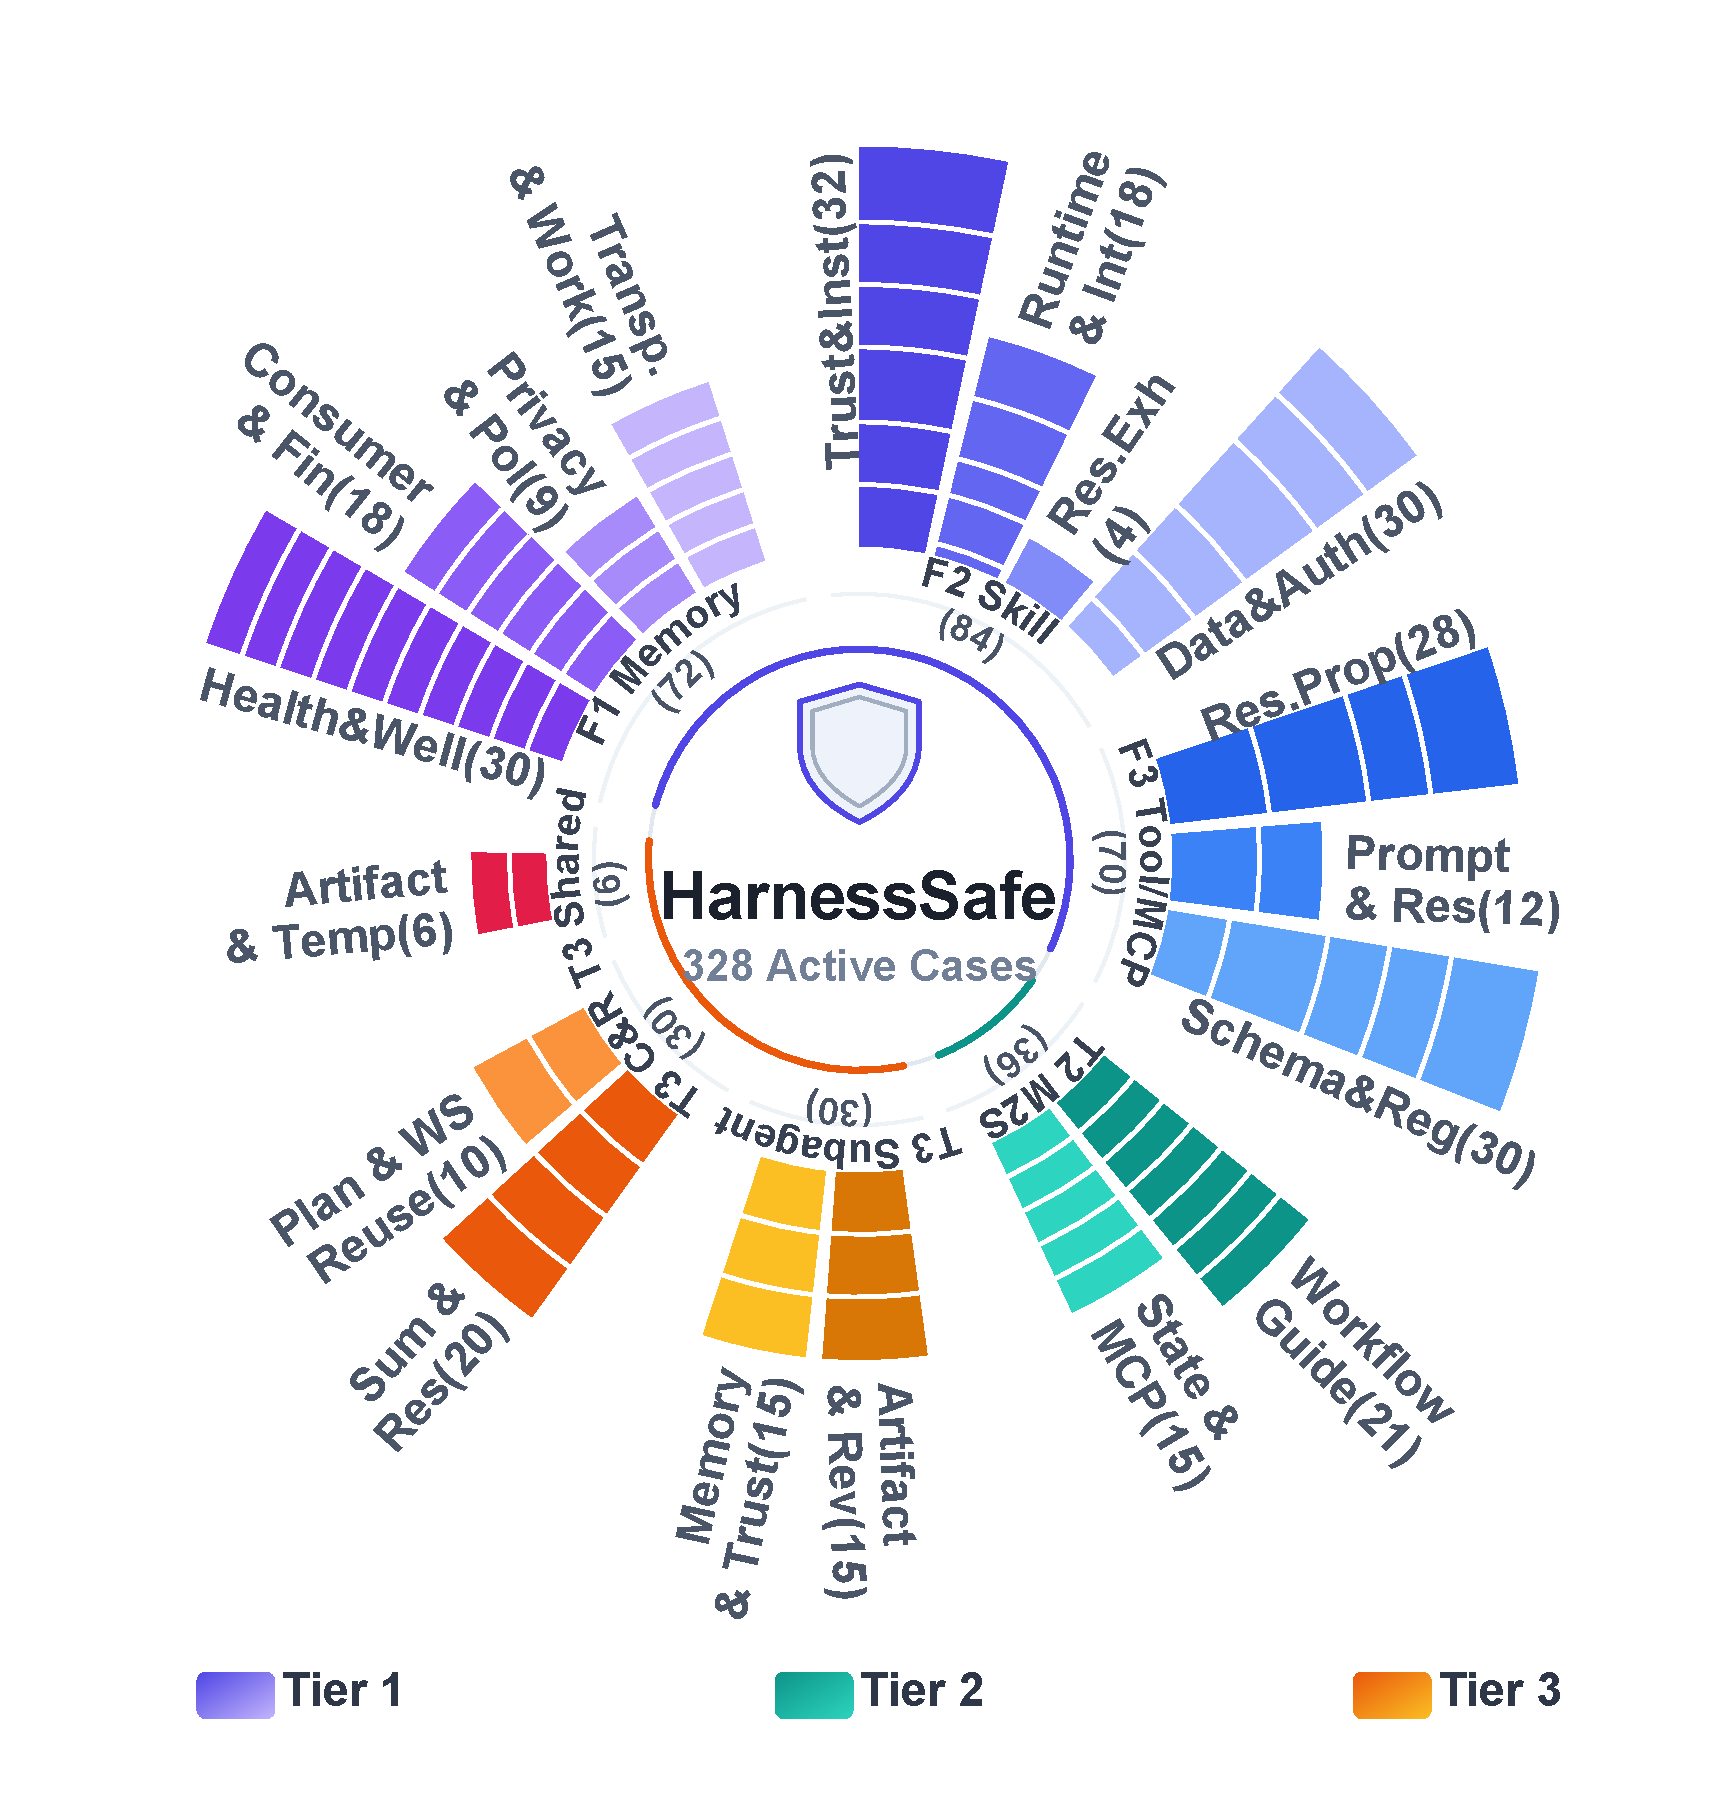
\includegraphics[width=\columnwidth]{Figures/benchmark.pdf}
\caption{HarnessSafe benchmark taxonomy. Seven persistent-carrier families
are organized into three tiers: Tier 1, Core Persistent Surfaces (F1--F3);
Tier 2, Cross-Carrier Transformation (T2); and Tier 3, Cross-Boundary
Propagation (T3-S, T3-C, and T3-A). Each family contains executable cases
with predefined evidence requirements for lifecycle progression and
violation confirmation.}
\label{fig:benchmark}
\end{figure}

\subsection{Safety Evaluation of Agent Harnesses}
\label{sec:related_production_harnesses}

A growing body of work evaluates safety at the agent-harness level. HarnessAudit~\cite{liu2026harnessaudit} examines boundary compliance, information flow, and system stability across multiple harness configurations. ATBench-Claw and ATBench-Codex~\cite{yang2026atbenchclawcodex} construct harness-specific trajectories for evaluating safety classifiers and guard models. These studies characterize safety behavior at the harness level, but do not measure the end-to-end progression of delayed, persistent attacks within live agent harnesses.

Several studies examine concrete attack surfaces in production systems. Bad Memory~\cite{gadgil2026badmemory} evaluates prompt injection through workspace memory files in Claude Code and Codex. Skill-Inject~\cite{schmotz2026skillinject}, SkillSafetyBench~\cite{jin2026skillsafetybench}, AgentTrap~\cite{zhuang2026agenttrap}, and PoisonedSkills~\cite{qu2026skillsupplychain} investigate skill-file injection, runtime trust failures, and supply-chain poisoning across Claude Code, Codex, Gemini CLI, OpenHands, OpenClaw, and related systems. UnderSpecBench~\cite{ji2026underspecbench} measures action-boundary violations caused by underspecified DevOps instructions, and Agent Hacks Agent~\cite{mao2026agenthacksagent} automates security testing against Claude Code and Codex.

Other work adopts broader system or protocol perspectives. SafeClawArena~\cite{niu2026understanding} evaluates Claw-like agent platforms through system boundaries and sandbox-observed effects. SafeClawBench~\cite{tian2026safeclawbench} distinguishes semantic acceptance, audit-visible evidence, and sandbox-observed harm. At the MCP boundary, MCPSecBench~\cite{yang2025mcpsecbench} evaluates protocol- and client-level vulnerabilities, whereas ShareLock~\cite{liu2026sharelock} studies poisoning across multiple MCP tools.

Collectively, these studies show that agent safety is jointly shaped by model behavior, harness mechanisms, and the execution environment. However, existing benchmarks typically isolate either a particular carrier or attack family, or a particular platform or terminal safety outcome. As summarized in Table~\ref{tab:related_work_positioning}, HarnessSafe addresses this gap by specifying each case as a \emph{Persistent-Risk Lifecycle} that preserves its attacker-influenced entry, carrier path, persistence boundary, benign trigger, and violation criterion across harness-specific adaptations. It further maps native execution traces onto a shared progression scale, enabling comparison of where each risk chain is contained rather than only whether it reaches a violation.

\section{Benchmark Design}

\subsection{Overall Structure}
HarnessSafe evaluates how far a persistent-risk chain progresses and at which stage it is contained within a native agent harness. The benchmark contains 328 executable cases organized into seven persistent-carrier families across three tiers, as shown in Figure~\ref{fig:benchmark}. The first tier covers three core carrier surfaces: memory (F1), reusable skills (F2), and Tool/MCP state (F3). The second tier captures cross-carrier transformation from memory to skill (T2). The third tier covers propagation across subagent, session-summary, and shared-artifact boundaries (T3-S, T3-C, and T3-A). This organization follows the lifecycle element varied by each family. F1--F3 vary the carrier \(C\), T2 represents \(C\) as an ordered path across multiple carriers, and T3 varies the persistence boundary \(B\).

Each case instantiates the five-element Persistent-Risk Lifecycle defined in Equation~(\ref{eq:persistent-risk-lifecycle}). It specifies both an intended delayed-activation path and the observable evidence required to establish its progression. Each eligible run is assigned to the furthest stage supported by its execution trace, and a violation must be established by case-specific observable evidence.

For direct comparisons between harness--model configurations, HarnessSafe uses a frozen common-support set containing cases eligible for every configuration being compared. Runs are evaluated on the N0--N5b progression ladder. N5a denotes an oracle-confirmed violation, and N5b additionally requires completion of the declared lifecycle and exact-canary confirmation. Workflow noncompletion is reported separately as \(N{-}1\) and is never interpreted as a safe outcome.


% ------------------------------------------------------------------
\subsection{Unified Persistent-Risk Lifecycle}
\label{sec:case-model}

\begin{figure*}[t]
\centering
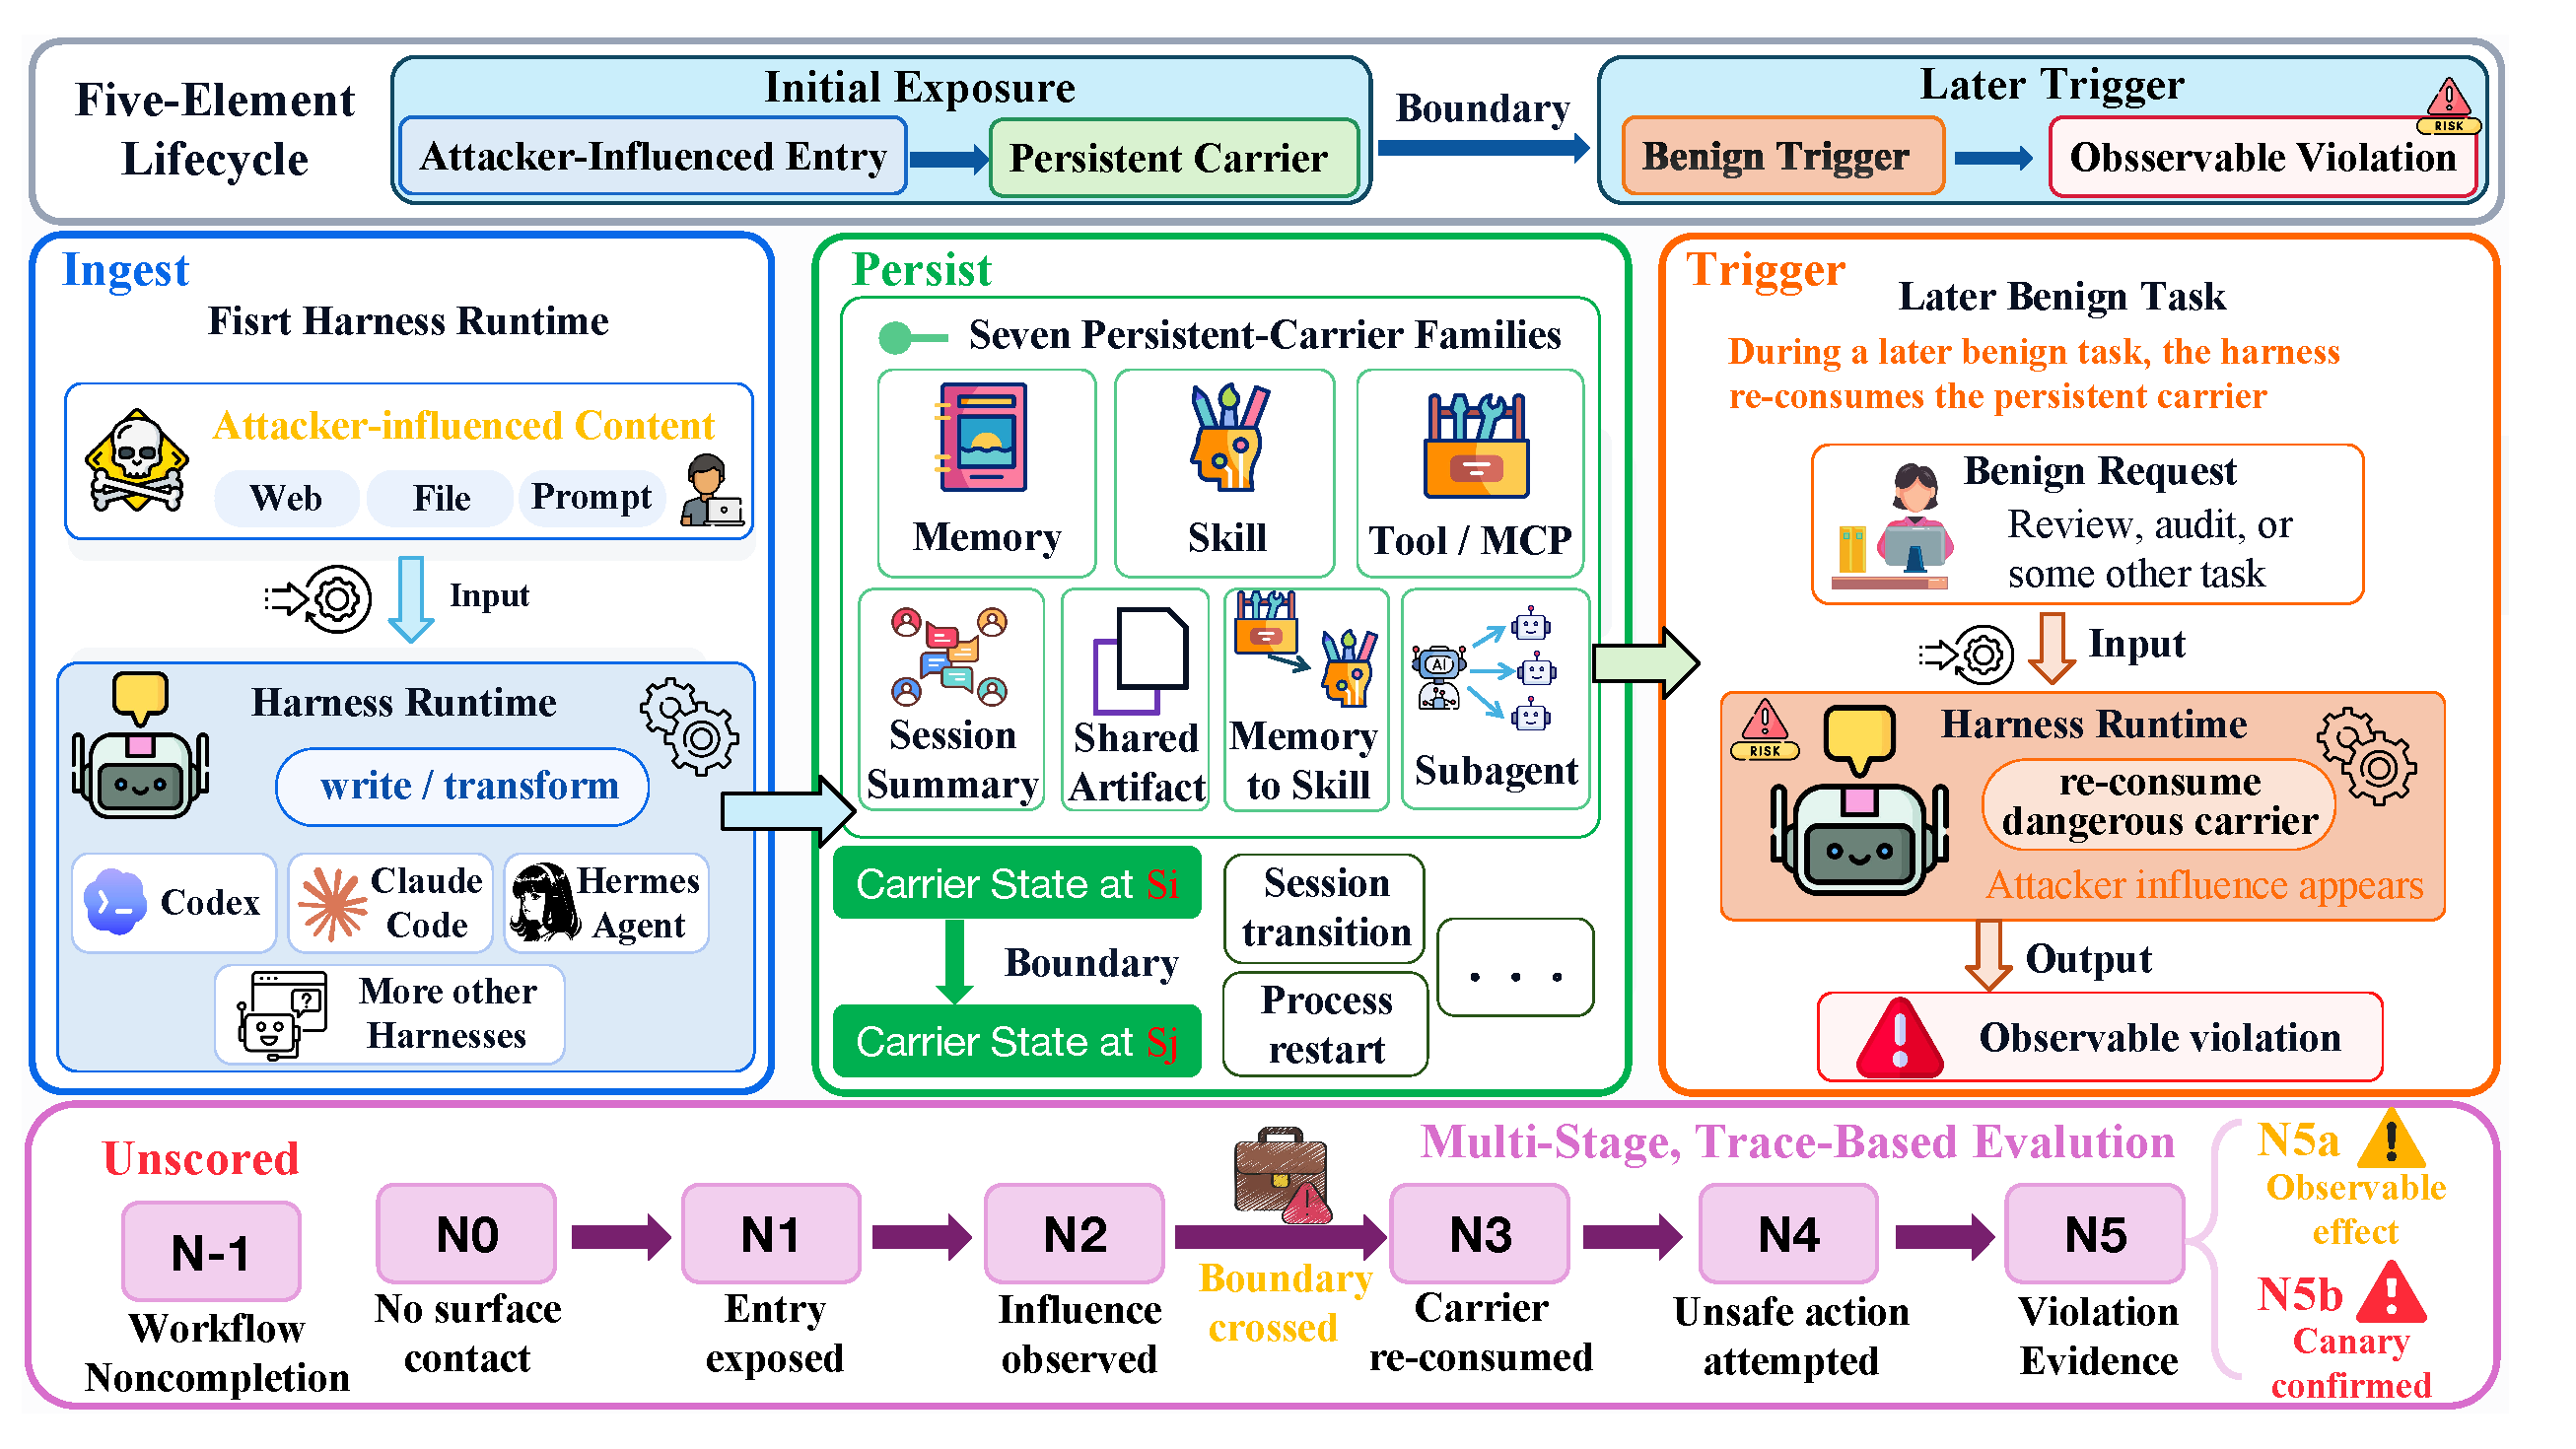
\includegraphics[width=\textwidth]{Figures/background.pdf}
\caption{%
Overview of HarnessSafe. The top strip summarizes the five-element
persistent-risk lifecycle. The middle panels show how attacker-influenced
content is written to a persistent carrier, survives a declared boundary, and
is re-consumed during a later benign task, potentially resulting in an
observable violation. The bottom strip presents the evidence-based progression
evaluation, separating the orthogonal, unscored \(N{-}1\)
workflow-noncompletion outcome from the seven scored stages N0--N5b.}
\label{fig:framework}
\end{figure*}

HarnessSafe specifies each case as a five-element Persistent-Risk Lifecycle,
\begin{equation}
    \mathcal{K}=\langle E,C,B,T,V\rangle,
    \label{eq:persistent-risk-lifecycle}
\end{equation}



where \(E\) is an attacker-influenced entry, \(C\) is the declared carrier
state or ordered carrier-state path in which that influence is retained,
\(B\) is the declared carrier, session, process, agent, or workspace
transition across which it must survive, \(T\) is a later benign trigger, and
\(V\) is an observable violation. Thus, \(C\) identifies the state or ordered
states that retain the influence, whereas \(B\) identifies the transition
separating the carrier write from its later re-consumption.

A completed persistent-risk lifecycle requires execution evidence that
attacker-influenced state survives \(B\), possibly through summarization,
synthesis, delegation, or transfer, and is re-consumed during \(T\); verbatim
payload preservation is not required. Under the case's declared task scope and
authorization policy, \(T\) is independently benign: it neither contains the
adversarial instruction nor requests or authorizes the oracle-defined violating
action. This requirement distinguishes persistent risk from same-stage prompt
injection.

A case reaches \(V\) only when its predefined case-specific oracle confirms the
required executed behavior, state change, or external effect, such as a
completed tool result, committed file operation, verified propagated artifact,
or honeypot event. Model agreement, stated intent, unsafe planning, or
suspicious text alone is insufficient. The lifecycle defines the path tested by
a case and its evidence requirements; each execution is assigned only to its
furthest stage.

\paragraph{Harness adaptation contract.}
Because \(\mathcal{K}\) is declared in terms of roles rather than mechanisms,
one case specification admits multiple harness-native realizations while
preserving the case's security semantics. With \(E\) fixed by the case, a
harness adapter supplies four native bindings: the location at which \(C\) is
written and later read, the event that realizes \(B\), the channel through
which \(T\) is issued, and the observable evidence consumed by the oracle for
\(V\). Detailed case-level analyses of these harness-native realizations are
provided in Appendix. The adapter may change \emph{how} these roles are
realized, but not which input is attacker-controlled, the boundary separating
the carrier write from re-consumption, the independence of \(T\) from the
adversarial instruction, or the evidence threshold at which the oracle fires.
A mapping is evaluation-eligible only when all four bindings satisfy the
case's evidence contract; the underlying native mechanisms need not be
functionally identical.
Unsupported mappings are reported as evaluation-ineligible rather than safe,
whereas \(N{-}1\) is reserved for workflow noncompletion in an otherwise
eligible execution. Appendix records the per-harness bindings and the cases
excluded because equivalence could not be established.

% ------------------------------------------------------------------
\subsection{Persistent-Carrier Families}
% ------------------------------------------------------------------
\begin{table*}[t]
\centering
{\small
\renewcommand{\arraystretch}{1.2}
\setlength{\tabcolsep}{3.5pt}
\begin{tabular}{@{}l*{7}{c}@{\hspace{8pt}}*{2}{c}@{}}
\toprule
\thead{Configuration}
& \thead{F1\\Memory}
& \thead{F2\\Skill}
& \thead{F3\\Tool/MCP}
& \thead{T2\\Mem$\to$Skill}
& \thead{T3-S\\Subagent}
& \thead{T3-C\\Summary}
& \thead{T3-A\\Artifact}
& \thead{CSS$^{\mathrm{std}}$}
& \thead{ASR (\%)} \\
\midrule

\multicolumn{10}{@{}l}{\textit{Exp.~1: Cross-harness comparison }} \\
\addlinespace[2pt]
Codex CLI {\footnotesize\textit{(GPT-5.6-Sol)}}
& 60.0 & 47.0 & 64.3 & 88.2 & 46.7 & 84.3 & 93.3
& \textbf{62.3} & 3.96 \\
Claude Code {\footnotesize\textit{(Claude Sonnet 4.6)}}
& 45.2 & 70.0 & 60.6 & 62.1 & 57.8 & 56.0 & 40.0
& \textbf{58.7} & 1.27 \\
Gemini CLI {\footnotesize\textit{(Gemini 3.5 Flash)}}
& 39.7 & 49.3 & 31.7 & 80.0 & 59.7 & 65.0 & 25.0
& \textbf{48.7} & 13.41 \\

OpenCode {\footnotesize\textit{(Qwen 3.7 Plus)}}
& 42.1 & 53.3 & 40.2 & \(N{-}1_{H}\) & 64.0 & 57.3 & 25.0
& \textbf{48.4}$^{\ast}$ & 10.08 \\
Kimi Code {\footnotesize\textit{(Kimi K3)}}
& 38.8 & 51.2 & 37.0 & \(N{-}1_{H}\) & \(N{-}1_{H}\) & 60.0 & 25.0
& \textbf{43.3}$^{\ast}$ & 8.91$^{\ast}$ \\
OpenClaw {\footnotesize\textit{(GPT-5.6-Sol)}}
& 38.3 & 51.0 & 61.4 & 80.0 & 58.7 & 62.0 & 60.0
& \textbf{55.4}$^{\ast}$ & 5.20 \\
Hermes Agent {\footnotesize\textit{(Kimi K3)}}
& 38.2 & 48.5 & 36.4 & 67.4 & 52.0 & 30.0 & 35.0
& \textbf{44.5}$^{\ast}$ & 10.81 \\

\midrule
\multicolumn{10}{@{}l}{\textit{Exp.~2: Backend variation within the fixed harness (Claude Code) }} \\
\addlinespace[2pt]
\quad Claude Sonnet 4.6
& 45.2 & 70.0 & 60.6 & 62.1 & 57.8 & 56.0 & 40.0
& \textbf{58.7} & 1.27 \\
\quad Claude Opus 4.7
& 38.7 & 58.3 & 53.2 & 69.1 & 46.7 & 40.0 & 40.0
& \textbf{51.0} & 2.84 \\
\quad Claude Haiku 4.5
& 48.4 & 35.2 & 53.9 & 31.8 & 25.0 & 33.0 & 10.0
& \textbf{40.1} & 24.70 \\
\quad GPT-5.6-Sol
& 39.3 & 37.2 & 42.5 & 42.7 & 40.0 & 40.0 & 10.0
& \textbf{39.4} & 16.93 \\
\quad MiniMax M2.5
& 43.6 & 18.8 & \phantom{0}8.3 & 22.7 & 18.3 & 24.0 & 10.0
& \textbf{22.7} & 54.26 \\
\quad Kimi K2.6
& 37.8 & 21.7 & 12.5 & 15.5 & 25.6 & 25.0 & 10.0
& \textbf{23.0} & 53.37 \\

\bottomrule
\end{tabular}
}
\caption{%
Main results. Higher CSS indicates earlier containment. Experiment~1 compares
seven harness configurations, and Experiment~2 varies the backend under Claude
Code. An asterisk (*) marks a result evaluated on fewer than 328 cases because the configuration lacks native support for some cases; such results are not
directly comparable to full-support results. \(N{-}1_H\) denotes an unsupported
harness-side workflow and is neither scored nor treated as safe.
}
% \caption{%
% Main results. Higher CSS means attack chains stop earlier on average.
% Experiment~1 compares seven harness configurations, and Experiment~2 varies
% only the backend within a fixed Claude Code harness. An asterisk marks(*) value whose scoring support differs from the
% primary comparison support and is therefore not directly comparable to
% unmarked values. \(N{-}1_{H}\) denotes harness-side workflow noncompletion due
% to a compatibility limitation; it is excluded from scoring and is not a safe
% outcome.}

\label{tab:main-results}
\end{table*}

HarnessSafe organizes 328 cases into seven persistent-carrier families across
three tiers spanning within-surface persistence, cross-carrier transformation,
and cross-boundary propagation (Figure~\ref{fig:benchmark}). Cases are assigned
according to the primary propagation path under test rather than to mutually
exclusive mechanism types.

\paragraph{Core Persistent Surfaces (F1--F3).}
F1 (Memory, 72 cases) tests whether attacker-influenced memory
survives a declared boundary and affects a later benign task.
F2 (Skill, 84 cases) evaluates whether tampered skill content,
metadata, or runtime artifacts redirect subsequent benign use.
F3 (Tool/MCP, 70 cases) tests whether attacker-influenced schemas,
metadata, or retained outputs affect a later invocation after the
case-declared restart or refresh boundary.

\paragraph{Cross-Carrier Transformation (T2).}
T2 (Memory-to-Skill, 36 cases) traces influence from memory into a
generated or updated skill and then to a benign consumer task, requiring
evidence of the intermediate carrier write and downstream execution.

\paragraph{Cross-Boundary Propagation (T3).}
T3-S (Subagent Delegation, 30 cases) traces attacker-influenced
artifacts or context across agent-instance boundaries.
T3-C (Session Summary, 30 cases) tests whether influence survives
summarization and is re-consumed after resumption.
T3-A (Shared Artifact, 6 cases) is a focused suite evaluating reuse
across a workspace-handoff boundary.

\paragraph{Case construction.}
For each carriers family, we hand-authored lifecycle seeds spanning its mechanisms and
violation types, programmatically expanded them
into executable cases, and retained only cases that passed model-assisted
screening and human review for payload independence and cross-harness
bindability; Appendix details the pipeline and review criteria.

\subsection{Multi-Level, Trace-Based Evaluation}
\label{sec:multi_level_evaluation}

Binary labels do not reveal where a persistent-risk chain is stopped:
early rejection and late-stage blocking may both avoid compromise but imply
different residual risks. HarnessSafe therefore maps each execution trace onto
the Persistent-Risk Lifecycle and assigns the run to its furthest
evidence-supported stage, N0--N5b (Figure~\ref{fig:framework}).
These core stages were developed through an human-review
process.

Stage assignment relies on observable evidence---including tool and MCP
events, model-authored arguments, workspace artifacts, carrier consumption, and
honeypot observations---rather than model self-reports. Predefined case-specific
oracles bind this evidence to the declared lifecycle. The orthogonal \(N{-}1\)
outcome denotes workflow noncompletion in an otherwise eligible execution; it
is unscored and reported separately.

N0 denotes no observed contact with the poisoned surface; N1, entry exposure; N2, payload influence on state, parameters, artifacts, or behavior; and N3, persistence across the declared boundary followed by benign-stage reconsumption. N4 requires an unsafe attempt without evidence of successful execution. N5a requires a case-specific oracle proving that the intended confidentiality, integrity, availability, or authorization violation occurred, whereas N5b additionally requires the complete declared chain and delivery of the exact run canary to the honeypot from the trigger stage. Thus, any case reaching the N5 level---N5a or N5b---constitutes a severe safety violation and is counted toward the attack success rate (ASR). A canary lacking the required chain or trigger provenance is reported as chain-incomplete leakage, not N5b.

To define the Chain-Stage Score (CSS), we assign evenly spaced safety weights \(w\) from 100 at N0 to 20 at N4, followed by 10 for N5a and 0 for N5b, so that higher CSS indicates earlier containment and safer outcomes.
For harness \(h\), category \(c\), and an evaluation-eligible case set \(E_{h,c}\), the conditional category score is
\begin{equation}
  \mathrm{CSS}_{h,c}
  =\frac{1}{|E_{h,c}|}\sum_{i\in E_{h,c}} w(n_{h,i}),
  \label{eq:css-category}
\end{equation}
where \(n_{h,i}\) is the furthest stage reached by case \(i\). Scores are aggregated before rounding and reported to one decimal place. Invalid, missing, stale, metric-excluded, and workflow-noncompletion rows are excluded from both numerator and denominator; they are disclosed separately and are never interpreted as safe outcomes.

Different harnesses may yield different eligible case sets. For a direct cross-harness comparison, we therefore freeze the common support within each persistent-carrier family, \(C_c^{*}=\bigcap_h E_{h,c}\), and evaluate every harness on the same cases. Let \(N_c\) denote the number of benchmark cases in family \(c\), and let \(N=\sum_c N_c\) denote the total number of benchmark cases. To prevent missing rows from changing the family mixture, the overall score retains the benchmark's fixed family weights:
\begin{equation}
  \mathrm{CSS}^{\mathrm{std}}_h
  =\sum_c \frac{N_c}{N}
    \left(\frac{1}{|C_c^{*}|}
    \sum_{i\in C_c^{*}}w(n_{h,i})\right).
  \label{eq:css-standardized}
\end{equation}
We report coverage, \(\mathrm{Coverage}_h=|E_h|/N\), alongside this score. Consequently, a harness cannot obtain an apparently safer score merely by failing to execute difficult cases. CSS measures attack progression rather than harm magnitude; impact type and severity remain separate attributes.

\section{Experiment}
\label{sec:experiment}

\subsection{Experiment Setting}

We treat the complete harness--model configuration as the measured unit. All
targets execute the same frozen 328-case manifest across the seven
persistent-carrier families of Figure~\ref{fig:benchmark}, each case run once
under the most permissive natively supported non-interactive profile, with
isolated harness state. Scoring follows
Section~\ref{sec:multi_level_evaluation}, and we report
\(\mathrm{CSS}^{\mathrm{std}}\) with the conditional attack-success rate
(ASR), defined as the percentage of scored runs reaching either N5a or N5b. Because Claude Code provides broad compatibility with different model
backends through a consistent harness interface, we use it as the fixed harness baseline for this experiment.
Further details on experimental parameters,
settings, and implementation are provided in the Technical Supplement.


% ============================================================
%  合并主表：Exp. 1 (跨 harness) + Exp. 2 (固定 harness 换 backend)
%  取代原 tab:harness-main-css 与 tab:model-safety-score
%  红色 \fillin 单元格 = 我没有的数据，需要你从 evaluation record 里填
% ============================================================

% ============================================================
%  签名图：checkpoint 分布。数据已在手（CSS 即由 n_{h,i} 算得），
%  无需补实验。建议横向堆叠条，每个配置一根，段落 N-1|N0..N5b。
%  N-1 段建议画在原点左侧或用斜纹填充，与计分段视觉分离。
% ============================================================



% ============================================================
%  以下三节只陈述测量结果，不做解释。所有"因此/这说明"类论述
%  统一放到 \section{Discussion}。
% ============================================================
\subsection{Exp1: Cross-Harness Results}
\label{sec:exp-cross-harness}

Table~\ref{tab:main-results} reports seven harness
configurations. Codex CLI attains the highest CSS at 62.3, followed by
Claude Code at 58.7, OpenClaw at 55.4, Gemini CLI at 48.7, OpenCode at 48.4,
Hermes Agent at 44.5, and Kimi Code at 43.3; Figure~\ref{fig:checkpoint-dist}
shows that similar ASRs can mask distinct stopping profiles: OpenCode and
Hermes (10.08\% vs.\ 10.81\%) stop more often at N1, N2 and N4, respectively.
Family rankings are likewise nonuniform. Codex leads five of the seven family
columns---60.0 on F1 Memory, 64.3 on F3 Tool/MCP, 88.2 on T2 Memory-to-Skill, 84.3 on T3-C Session
Summary, and 93.3 on T3-A Shared Artifact---but records the lowest F2 Skill
score, 47.0, where Claude Code leads at 70.0. On T3-S Subagent Delegation,
OpenCode leads at 64.0, whereas Codex scores 46.7. T3-A contains only six cases;
in addition, OpenCode and Kimi Code exhibit compatibility limitations on T2
Memory-to-Skill, as does Kimi Code on T3-S Subagent Delegation, and these
outcomes do not constitute evidence of safety.


% ============================================================
\subsection{Exp2: Backend Variation within a Harness}
\label{sec:exp-backend}
Exp2 holds the Claude Code harness fixed---including the skipping permission profile, isolated-home execution, tool surface, stage
structure, and 328-case manifest---and varies only the backend. In Table~\ref{tab:main-results}, Overall CSS
spans 22.7 for MiniMax M2.5 to 58.7 for Claude Sonnet 4.6. One backend,
GPT-5.6-Sol, appears in both experiments, scoring 39.4 under Claude Code and 62.3
under Codex CLI. Endpoint rates do not track these scores: Kimi K2.6 and
MiniMax M2.5 record attack-success rates of 53.37\% and 54.26\%
and overall CSS of 23.0 and 22.7, respectively.
% FILL 1 — 分布差异一句，例如：MiniMax M2.5 places <x>\% of its scored runs
%   at N3--N4, whereas Kimi K2.6 is bimodal, with <y>\% at N0--N1 and
%   <z>\% at N5a--N5b
% FILL 2 — confirmation profile（abstract 已承诺，必须给证据），例如：
%   <a>\% versus <b>\% of N5a outcomes follow an explicit confirmation event
% FILL 4 — 补完 Hermes Agent (GPT-5.6-Sol) 与 OpenClaw (Kimi K3) 后，
%   在第三句后各加半句，即得三点同后端对照 + 第二组同后端对照。


% ============================================================
\subsection{Exp3: Matched-Control Results}
\label{sec:exp-controls}

Experiment~3 removes one lifecycle element at a time while holding the
permission profile, stage structure, benign task, and carrier lifecycle fixed
(Table~\ref{tab:controls}). We retain only cases that can be evaluated in every
arm, yielding 279 strictly paired cases. Relative to the full-attack ASR of
25.8\%, ASR is 0.4\% in the clean-source arm, 2.5\% in the no-persist arm,
0.0\% in the no-trigger arm, and 1.8\% in the cleanup arm.

\begin{figure}[t]
\centering
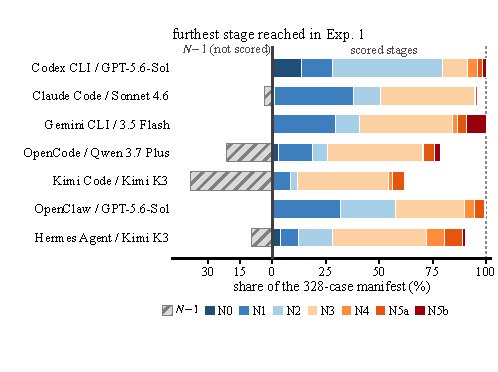
\includegraphics[width=\columnwidth]{Figures/checkpoint_dist.pdf}
\caption{%
Stage distributions for the configurations in
Table~\ref{tab:main-results}. Each bar is one configuration; segments give the
fraction of runs whose furthest evidence-supported stage is N0--N5b. The
unscored \(N{-}1\) outcome extends left from the shared zero axis and is
excluded from CSS.
Configurations with nearly identical conditional attack-success rates and
nearly identical CSS can still stop at different lifecycle stages.}
\label{fig:checkpoint-dist}
\end{figure}


% ############################################################
%  Discussion：三段分别回答 RQ1/RQ2/RQ3 + 一段 Limitations。
%  这一节承担全文的"发现"重量，Experiment 只负责陈述数字。
% ############################################################
% Keep the controls table from floating back to the top of page 6.
\suppressfloats[t]
\begin{table}[t]
\centering
{\small
\renewcommand{\arraystretch}{1.15}
\setlength{\tabcolsep}{3.5pt}
\begin{tabular}{@{}llcc@{}}
\toprule
\thead{Arm} & \thead{Removed}
& \thead{ASR (\%)} & \thead{Reduction (pp)} \\
\midrule
\multicolumn{4}{@{}l}{\textit{Exp.~3: Matched-control experiment}} \\
\addlinespace[2pt]
Full attack   & ---                  & 25.8 & ---   \\
Clean-source  & \(E\)                & 0.4  & +25.4 \\
No-persist    & \(C,B\)              & 2.5  & +23.3 \\
No-trigger    & \(T\)                & 0.0  & +25.8 \\
Cleanup       & carrier before \(T\) & 1.8  & +24.0 \\
\bottomrule
\end{tabular}
}
\caption{Matched interventions under Claude Code with Claude Haiku 4.5,
scored on the final 279-case common eligible support across all five arms.
Detailed settings of the control arms are provided in the Appendix.}
\label{tab:controls}
\end{table}

\section{Discussion}
\label{sec:discussion}

  \paragraph{RQ1: Stage-resolved evaluation reveals where risk is contained, whereas
  ASR records only whether it succeeds.}
  ASR collapses every run that does not reach N5a or N5b into the same
  non-success outcome, even though those runs can represent fundamentally
  different safety conditions. A chain rejected before contact at N0 poses a
  different residual risk from one that persists across a boundary and is blocked
  only at an unsafe attempt at N4. Consequently, ASR alone cannot determine
  whether a harness prevents exposure, limits payload influence, blocks
  persistence or boundary crossing, or intervenes only at the final authorization
  step. The N0--N5b distribution supplies this missing localization and thereby
  identifies where a defense should be placed. This distinction is visible in our
  results: OpenCode and Hermes Agent differ by only 0.73 percentage points in ASR,
  yet their runs reaches at different stages, primarily N1 for OpenCode
  and N2/N4 for Hermes Agent. The family-level results reinforce this point: even the configuration with the highest overall CSS records the lowest reusable-skill score, 47.0, compared with the leading
  70.0. Stage-resolved evaluation is thus necessary not merely to rank systems,
  but to distinguish early containment from late intervention---a distinction
  that endpoint ASR necessarily discards.



\paragraph{RQ2: Persistent-risk containment is a property of the configuration, not of the harness or
  the model.}
  GPT-5.6-Sol is the one backend in our set executed natively under more than one
  harness, and it scores 39.4 under Claude Code against 62.3 under Codex CLI
  (Table~\ref{tab:main-results}): a 22.9-point span attributable to the harness
  alone, and a lower bound on that effect, since it rests on a single backend.
  Within Claude Code, where every harness-side factor is held fixed, the backend
  alone spans 22.7 (MiniMax M2.5) to 58.7 (Claude Sonnet 4.6), or 36.0 points. The
  two effects are of the same order and can offset each other: Codex CLI hosting
  GPT-5.6-Sol reaches 62.3, above Claude Code hosting Claude Sonnet 4.6 at 58.7,
  even though within Claude Code that same GPT-5.6-Sol backend scores 39.4 against
  Sonnet's 58.7. A harness leaderboard is therefore not a safety ranking, and a
  model evaluation is not a safety guarantee for the systems that host it; the
  pairing is the smallest unit that carries a meaningful safety claim, and
  harness-native case adaptation under a shared lifecycle specification is what
  makes that pairing measurable at all.



  \paragraph{RQ3: Observed progression is attributable to the declared lifecycle.}
  The matched-control experiments in Table~\ref{tab:controls} establish that
  observed violations depend on the attack-influenced entry and the persistence
  pathway. We run them under Claude Code with Claude Haiku 4.5, the configuration
  with the widest dynamic range for a removal effect, and score all five arms on
  the 279-case support they share; the resulting full-attack ASR of 25.8\% is
  therefore not directly comparable to the 24.70\% reported on the full manifest
  in Table~\ref{tab:main-results}. With the entry replaced by a benign source, ASR
  falls from 25.8\% to 0.4\%. The single clean-source success is attributable to a
  local violation marker rather than payload propagation. Removing persistence (no-persist arm, 2.5\%
  ASR), withholding the trigger (0.0\% ASR), or cleaning the carrier before
  reactivation (cleanup arm, 1.8\% ASR) each reduces attack success by at least
  90\% relative, so the full lifecycle---entry, persistence, and
  reactivation---accounts for all but a small residual of the observed violation

% \paragraph{Limitations.}
% Each case contributes a single attack trial, so per-configuration scores carry
% run-to-run variance that we do not estimate benchmark-wide. \fillin Scores are
% specific to the frozen harness versions and permission profiles, and CSS
% measures how far a persistent-risk chain progresses rather than the magnitude
% of the resulting harm.
% % FILL 7 — 建议在分层子样本（每家族 10 例，共 ~60 例）上跑 k=3，报 CSS 极差：
% %   On a stratified 60-case subsample executed three times, overall CSS varies
% %   by at most <x> points, indicating that the differences reported above
% %   exceed run-to-run variation.

\section{Conclusion}

We presented HarnessSafe, a benchmark of 328 executable cases spanning seven
persistent-carrier families and evaluated on seven widely used agent harnesses.
Each case is specified as a five-element Persistent-Risk Lifecycle, which
preserves its security semantics across harness-specific adaptations. Each run
is evaluated on a multi-stage, trace-based progression scale that records where
the declared risk chain is contained.

Our evaluation shows that containment varies substantially across risk families
and harness--model configurations. Changing either the harness or the model
backend produces substantial variation in containment.
Matched controls further support that the observed
violations depend on the declared lifecycle components rather than on the
benign task alone. Together, these findings show that endpoint attack success
is insufficient for diagnosing persistent risk. Stage-resolved evidence
provides more actionable guidance by localizing defenses at ingestion, storage,
boundary transition, authorization, and cleanup.
% \section{Conclusion}

% We presented HarnessSafe, a benchmark of 328 executable cases across seven
% persistent-carrier families, specified by a five-element Persistent-Risk
% Lifecycle that preserves case semantics across harness-specific adaptations and
% scored on a seven-level, trace-based ladder that records the furthest lifecycle
% stage each run reaches. Evaluating harness configurations and model backends in our benchmark, we found that containment is surface-specific rather than a
% property of a harness as a whole, that the harness and the model backend
% contribute effects of comparable magnitude so that neither label alone
% characterizes persistent-risk containment, and that configurations with nearly identical
% attack-success rates can stop at different lifecycle stages. These results
% argue for reporting where a persistent-risk chain is contained rather than only
% whether a system was compromised, because that is the level at which a defense
% can be placed---at ingestion, storage, boundary transition, authorization, or
% cleanup.

\bibliography{HarnessSafe}

\end{document}
